\paragraph{}
We created a web application that allows us to browse and search in the Stackoverflow data using the Elasticsearch full-text queries. Furthermore, the application is ready for the integration of information retrieval techniques using the obtained vector representations of questions. In other words, the application will serve to demonstrate the benefits of this work, which is beyond the scope of this work.

\paragraph{}
In this appending, you can find screenshots (figures \ref{web_app_home} - \ref{question_2}) obtained from the application. Each screenshot is accompanied by a short caption with a description of the functionality. The purpose of the screenshots is to get an impression of how does the application work. A reader is not expected to read the text in the figures.

\begin{figure}[!h]
	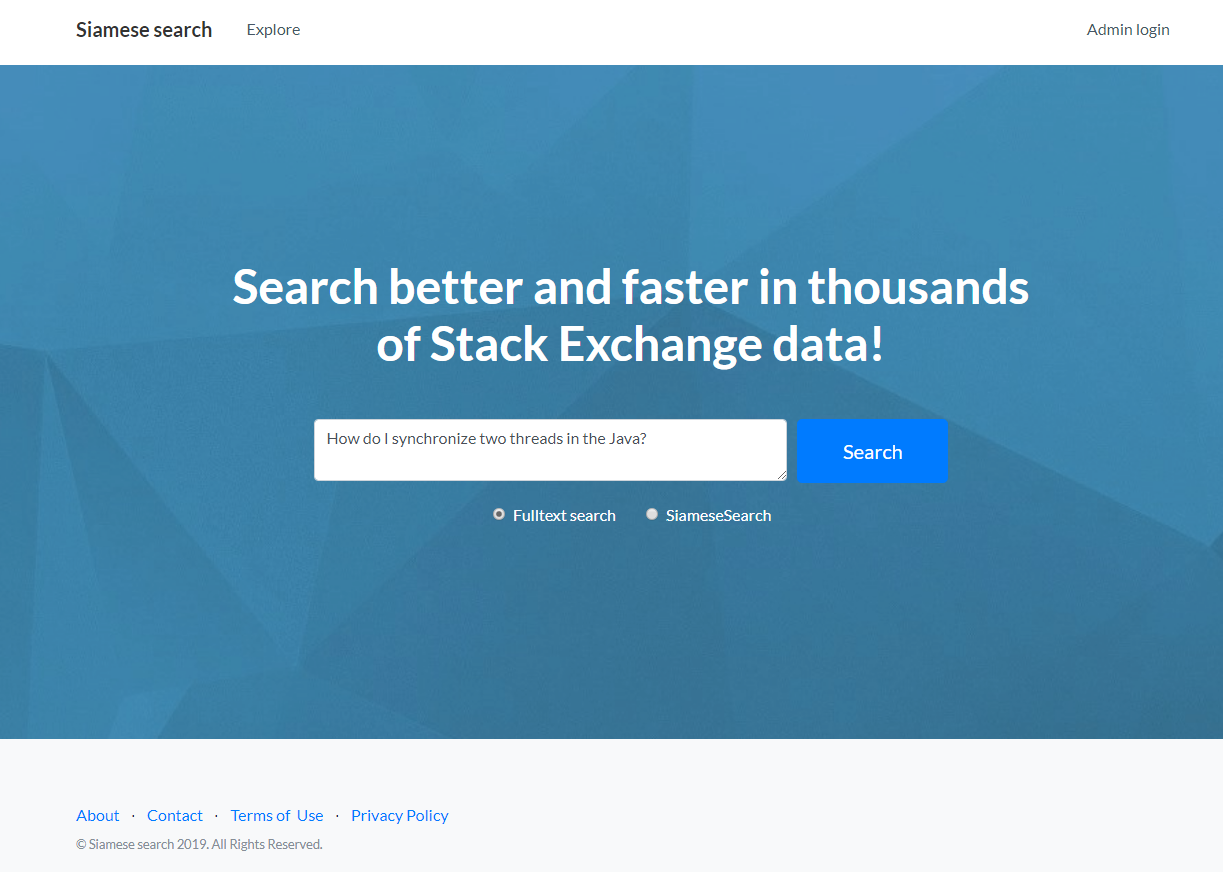
\includegraphics[width=19cm, angle=90]{web_app_home.PNG}
	\centering
	\caption{A homepage of the web application. In the middle of the screen, there is a text field for a query and a corresponding \textit{search} button. Users can select whether to use standard the full-text search or the improved search technique using our outcome. However, the latter is not implemented at the moment.}
	\label{web_app_home}
\end{figure}

\begin{figure}[!h]
	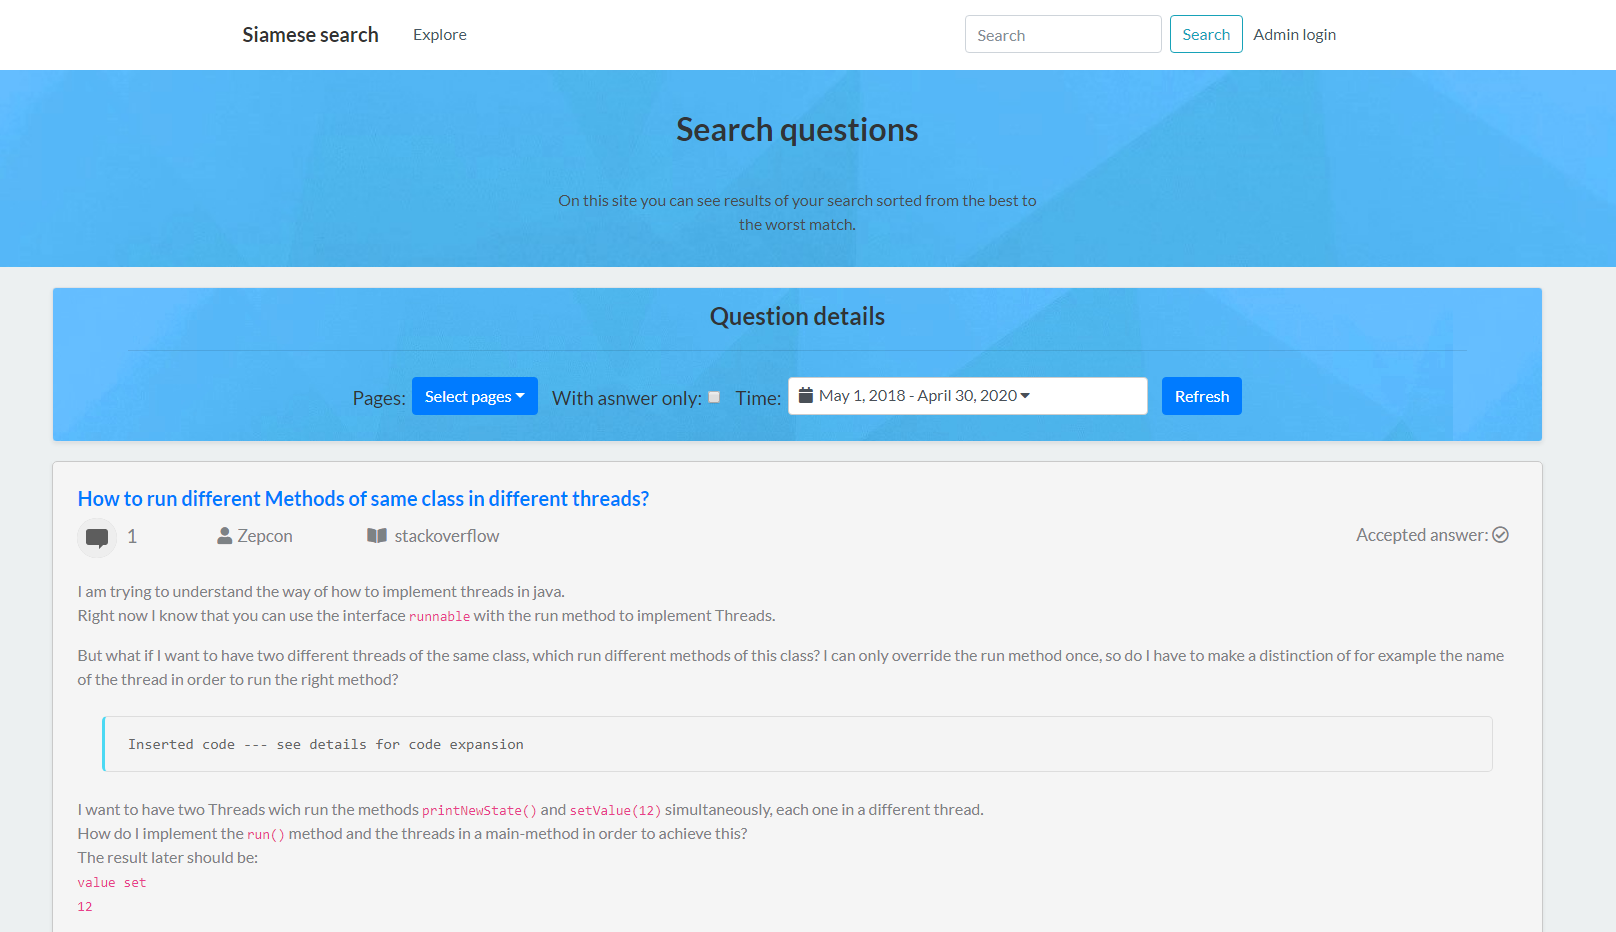
\includegraphics[width=20cm, angle=90]{search_res.PNG}
	\centering
	\caption{This figure shows a page with the results of the query displayed in figure \ref{web_app_home}. The page displays individual results with necessary information. Users can show details of the question by clicking the link in the title.}
	\label{search_res}
\end{figure}

\begin{figure}[!h]
	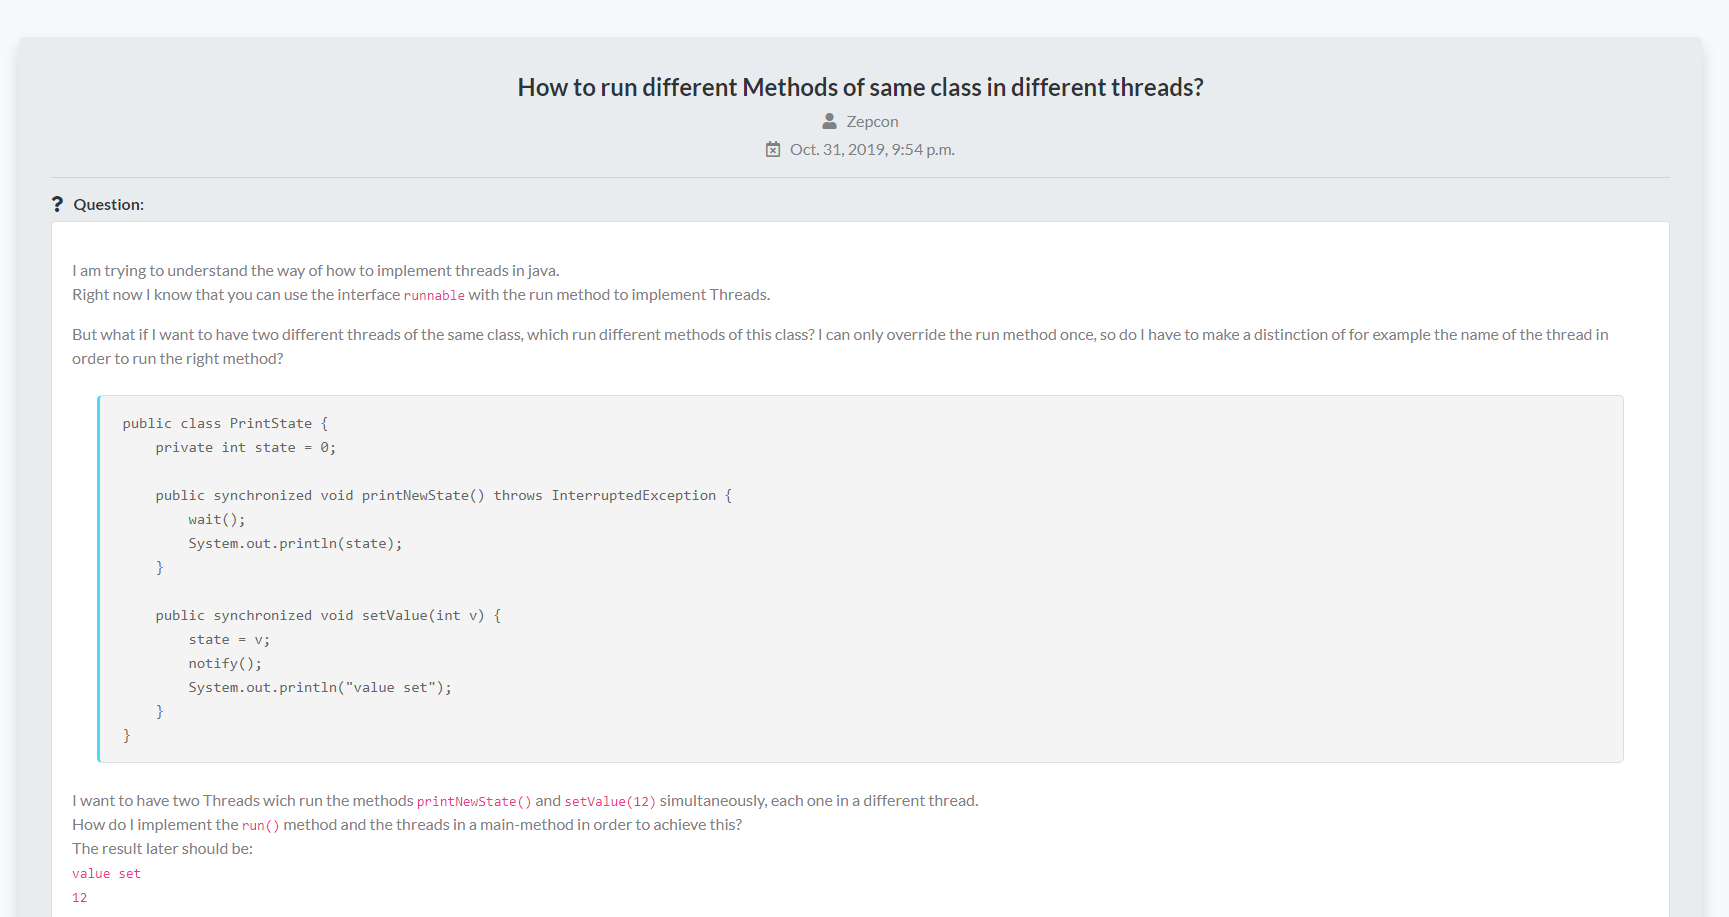
\includegraphics[width=20cm, angle=90]{question_1.PNG}
	\centering
	\caption{This figure shows a part of a page with details of the Stackoverflow question. On the top of the page, a title, author, and publish date is displayed. The question details are followed by expanded text and code snippet of the question.}
	\label{question_1}
\end{figure}

\begin{figure}[!h]
	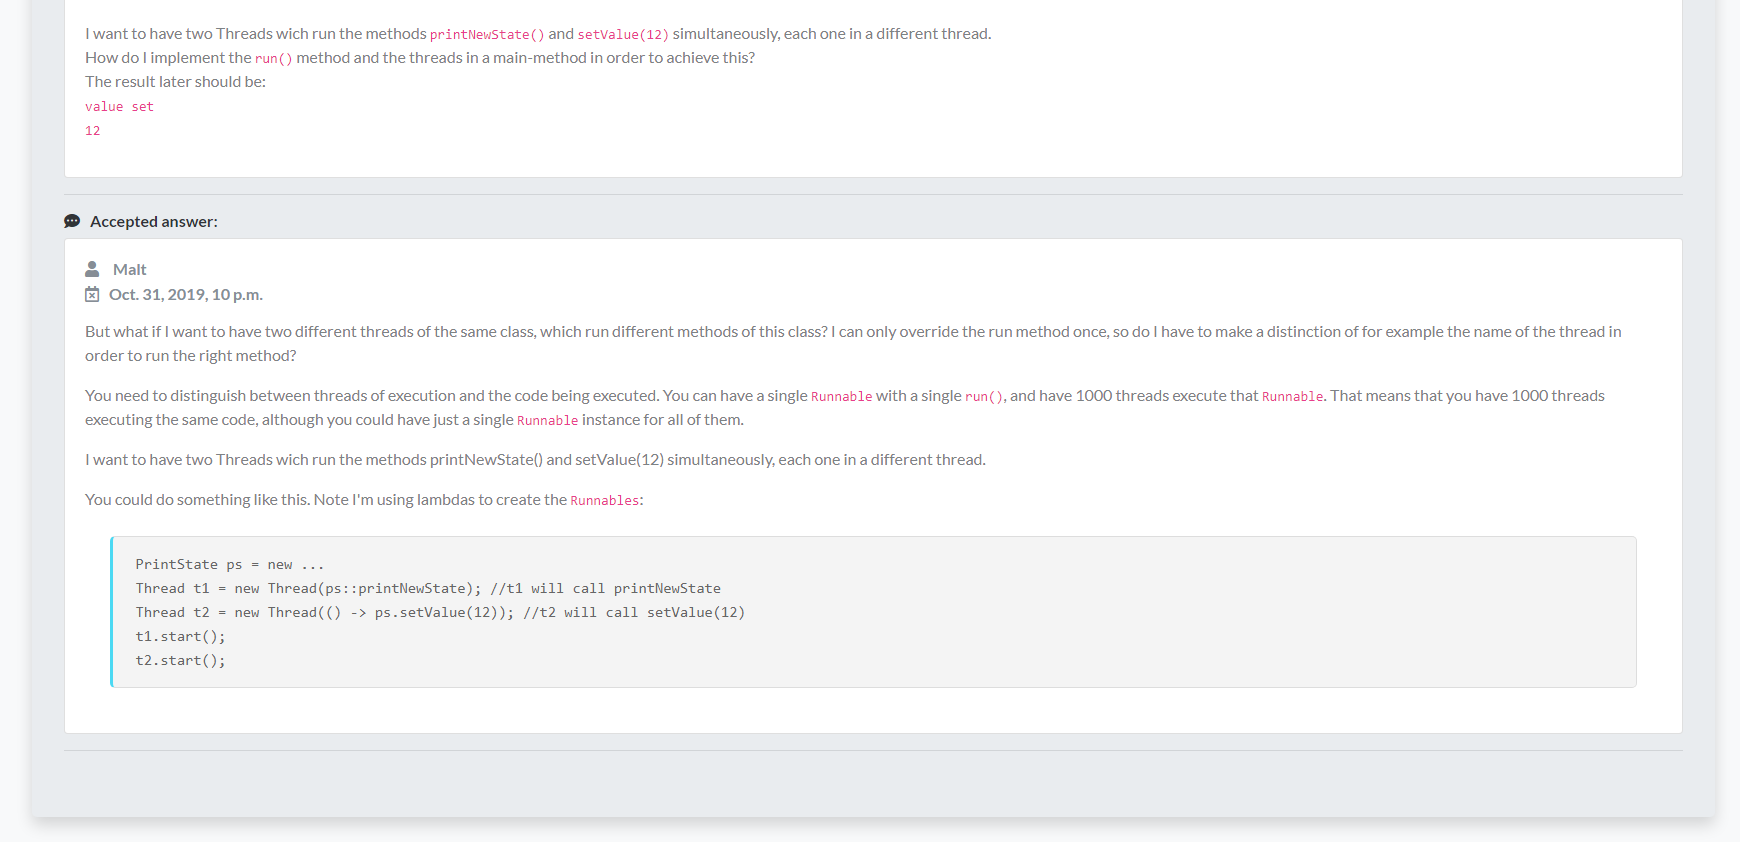
\includegraphics[width=20cm, angle=90]{question_2.PNG}
	\centering
	\caption{This figure follows the question details depicted in figure \ref{question_1}. In this part of the question detailed view, all answers and comments are displayed.}
	\label{question_2}
\end{figure}